\documentclass{report}
\usepackage[margin=1in, paperwidth=8.5in, paperheight=11in]{geometry}
%Math packages%
\usepackage{amsmath}
\usepackage{amsthm}
%Spacing%
\usepackage{setspace}
\onehalfspacing
%Lecture number%
\newcommand{\lectureNum}{12}
%Variables - Date and Course%
\newcommand{\curDate}{February 9, 2017}
\newcommand{\course}{CS 241}
\newcommand{\instructor}{Kevin Lanctot}
%Defining the example tag%
%\theoremstyle{definition}%
\newtheorem{ex}{Example}[section]
%Setting counter given the lecture number%
\setcounter{chapter}{\lectureNum{}}
%Package to insert code%
\usepackage{listings}
\usepackage{courier}
\usepackage{xcolor}
\lstset { %
    tabsize=2,
    breaklines=true,
    language=C++,
    backgroundcolor=\color{blue!8}, % set backgroundcolor
    basicstyle=\footnotesize\ttfamily,% basic font setting
}
%Package for images%
\usepackage{graphicx}

\begin{document}
%Note title%
\begin{center}
\begin{Large}
\textsc{\course{} | Lecture \lectureNum{}}
\end{Large}
\end{center} 
\noindent \textit{Bartosz Antczak} \hfill
\textit{Instructor: \instructor{}} \hfill
\textit{\curDate{}}
\rule{\textwidth}{0.4pt}
% Actual Notes%
\section{Scanning}
This applied to assignment 6, question 1.\\
The scanning for assembly language was fairly straightforward, but scanning high-level languages are more complicated. A scanner takes in input code (e.g., ``\texttt{i += 1}") and outputs a sequence of tokens.
\subsection{Scanning Approach}
We'll implement this scanner by reading in the file that contains the high-level language (which, recall, is a sequence of characters) and reading the file one character at a time.\\
The basic idea is to keep reading characters until you reach the error state:
\begin{enumerate}
\item check next state based on character $c_i$
\item If you reach an error (i.e., there doesn't exist a transition $c_i$ for the current state), look back at the previous state:
\begin{enumerate}
\item if it was not a final state, report error
\item if it was whitespace, ignore
\item if it was an accepting state, output the corresponding token
\item then go back to start state (i.e., begin looking for the next token)
\end{enumerate}
\end{enumerate}
The pseducode for this approach is:
\begin{figure}[ht]
\begin{center}
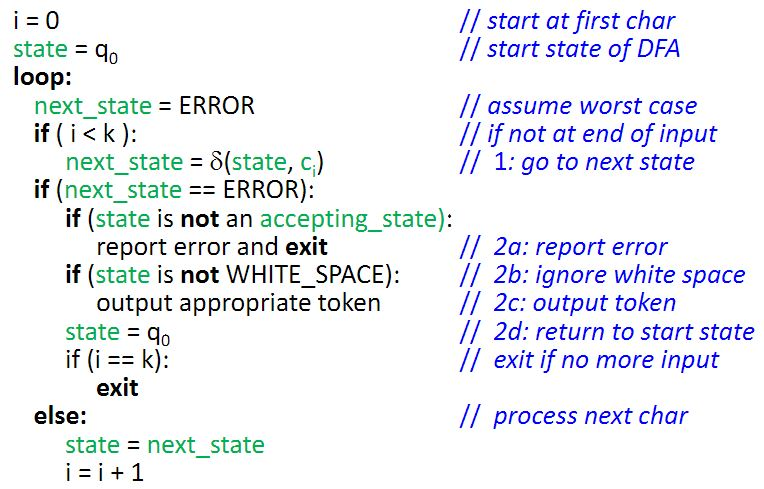
\includegraphics[scale=0.4]{scan1.jpg}
\end{center}
\caption{Courtesy of Prof. Lanctot's slides.}
\end{figure}\newpage
\section{Context-free Grammar}
We can now scan words and tokenize them in out programming language. What we have to do now if recognize the \textit{sentences} and their \textit{meaning}, this is called \textit{parsing}. We will now identify the syntax and semantics of the language. Right now, we'll focus on \textbf{syntax}.
\subsection{Current Challenge - Syntax}
Regular expressions, DFAs and NFAs aren't enough. We need something more powerful. For example, in any high-level language, we require balanced parentheses and balances braces:
\begin{center}
(()(())) $\qquad\qquad$ \{\{\{\}\}\}
\end{center}
The previous parentheses and braces are \textbf{balanced}. Unless if the difference between the left and right brace/parenthesis is fixed, it's impossible to create a DFA. Can you imagine if in C++ you can only create 3 nested \texttt{if} statements (because if there were more, the DFA wouldn't be able to read them)? That's ridiculous.\\When reading a line, we'll check if each token aligns properly with the token following it (e.g., if we have an integer, a semicolon is a possible accepting state that follows it). To determine if the tokens are aligned properly, we'll refer to a set of rules. For our WLP4 language, a set of rules is listed on WLP4 Language Specification  on the CS 241 website, under ``context-free syntax". The rules are structured such that if the current state leading to another state is included in the list, the it's valid. 
%END%
\end{document}